\begin{frame}{$BiFeO_{3}$ con arreglo antiferromagn\'etico tipo A}
            \begin{columns}[t]
        \column{0.5\textwidth}
        \begin{figure}[H]
            \centering
            \includegraphics[width=0.9\textwidth]{contenido/resultados/img_resultados/energia_BFO_A.png}
            \caption{Minimizaci\'on de la energ\'ia del $BiFeO_{3}$ con arreglo 
                antiferromagn\'etico tipo A.}
        \end{figure}
        \column{0.5\textwidth}
        \begin{figure}[H]
            \centering
            \includegraphics[width=0.9\textwidth]{contenido/resultados/img_resultados/fuerza_BFO_A.png}
            \caption{Minimizaci\'on de la fuerza del $BiFeO_{3}$ con arreglo 
            antiferromagn\'etico tipo A.}
        \end{figure}
    \end{columns}
\centering
\textbf{El sistema converge luego de 9 iteraciones.}
\end{frame}


\begin{frame}{$BiFeO_{3}$ con arreglo antiferromagn\'etico tipo G}
    \begin{columns}[t]
        \column{0.5\textwidth}
        \begin{figure}[H]
            \centering
            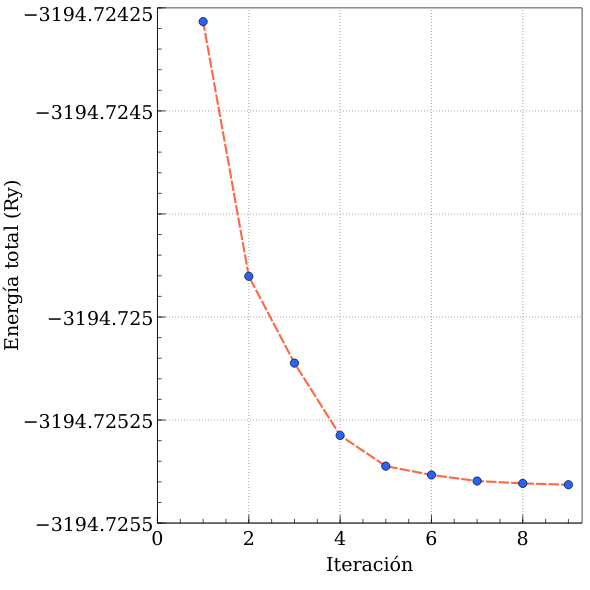
\includegraphics[width=0.9\textwidth]{contenido/resultados/img_resultados/energia_BFO_G.png}
            \caption{Minimizaci\'on de la energ\'ia del $BiFeO_{3}$ con arreglo 
                antiferromagn\'etico tipo G.}
        \end{figure}
        \column{0.5\textwidth}
        \begin{figure}[H]
            \centering
            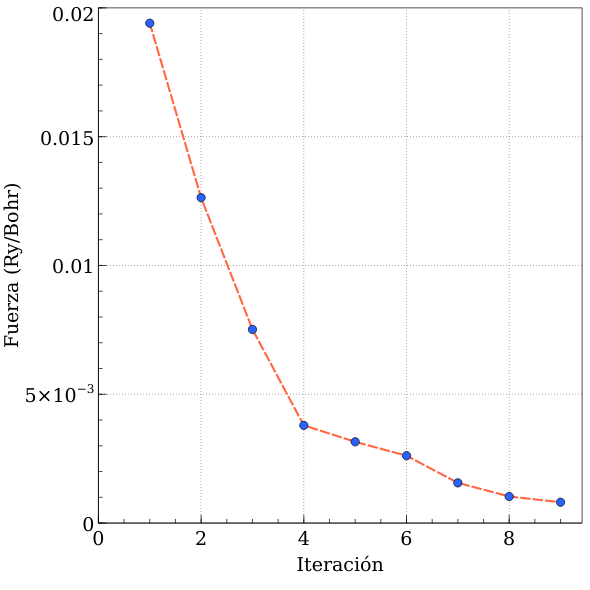
\includegraphics[width=0.9\textwidth]{contenido/resultados/img_resultados/fuerza_BFO_G.png}
            \caption{Minimizaci\'on de la fuerza del $BiFeO_{3}$ con arreglo 
                antiferromagn\'etico tipo G.}
        \end{figure}
    \end{columns}
\centering
\textbf{El sistema converge luego de 9 iteraciones.}
\end{frame}


\begin{frame}{$YCrO_{3}$ con arreglo antiferromagn\'etico tipo A}
    \begin{columns}[t]
        \column{0.5\textwidth}
        \begin{figure}[H]
            \centering
            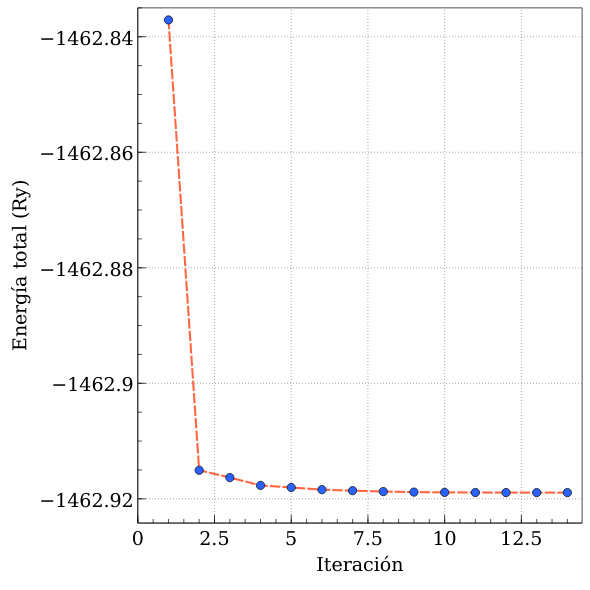
\includegraphics[width=0.9\textwidth]{contenido/resultados/img_resultados/energia_YCO_A.png}
            \caption{Minimizaci\'on de la energ\'ia del $YCrO_{3}$ con arreglo 
                antiferromagn\'etico tipo A.}
        \end{figure}
        \column{0.5\textwidth}
        \begin{figure}[H]
            \centering
            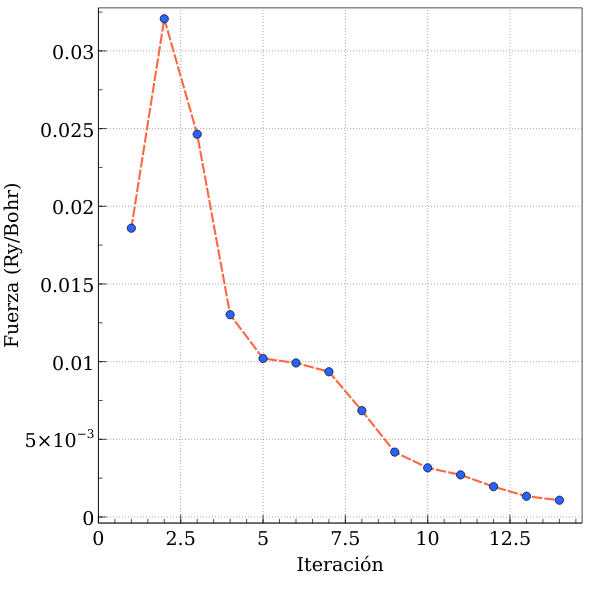
\includegraphics[width=0.9\textwidth]{contenido/resultados/img_resultados/fuerza_YCO_A.png}
            \caption{Minimizaci\'on de la fuerza del $YCrO_{3}$ con arreglo 
                antiferromagn\'etico tipo A.}
        \end{figure}
    \end{columns}
\centering
\textbf{El sistema converge luego de 14 iteraciones.}
\end{frame}


\begin{frame}{$YCrO_{3}$ con arreglo antiferromagn\'etico tipo C}
    \begin{columns}[t]
        \column{0.5\textwidth}
        \begin{figure}[H]
            \centering
            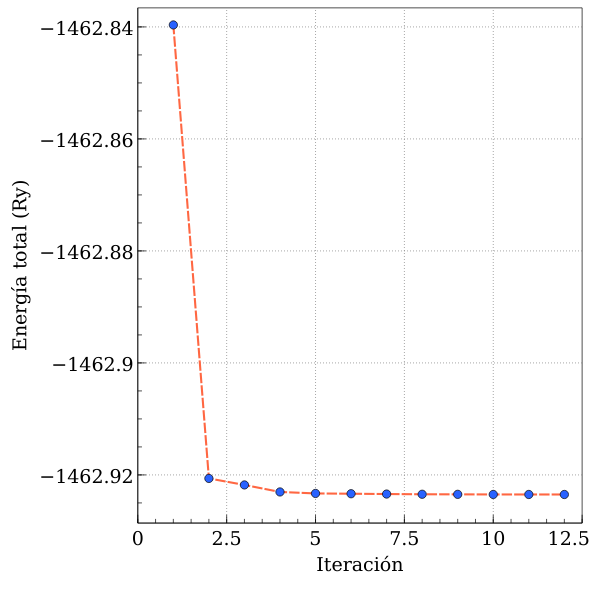
\includegraphics[width=0.9\textwidth]{contenido/resultados/img_resultados/energia_YCO_C.png}
            \caption{Minimizaci\'on de la energ\'ia del $YCrO_{3}$ con arreglo 
                antiferromagn\'etico tipo C.}
        \end{figure}
        \column{0.5\textwidth}
        \begin{figure}[H]
            \centering
            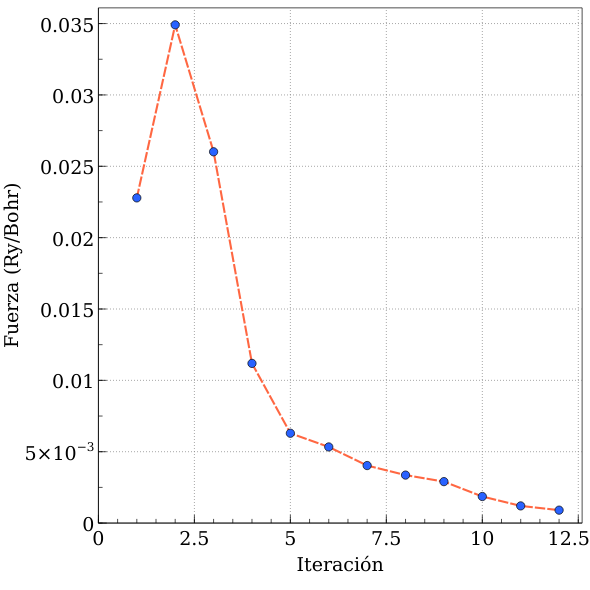
\includegraphics[width=0.9\textwidth]{contenido/resultados/img_resultados/fuerza_YCO_C.png}
            \caption{Minimizaci\'on de la fuerza del $YCrO_{3}$ con arreglo 
                antiferromagn\'etico tipo C.}
        \end{figure}
    \end{columns}
\centering
\textbf{El sistema converge luego de 12 iteraciones.}
\end{frame}


\begin{frame}{$YCrO_{3}$ con arreglo antiferromagn\'etico tipo G}
    \begin{columns}[t]
        \column{0.5\textwidth}
        \begin{figure}[H]
            \centering
            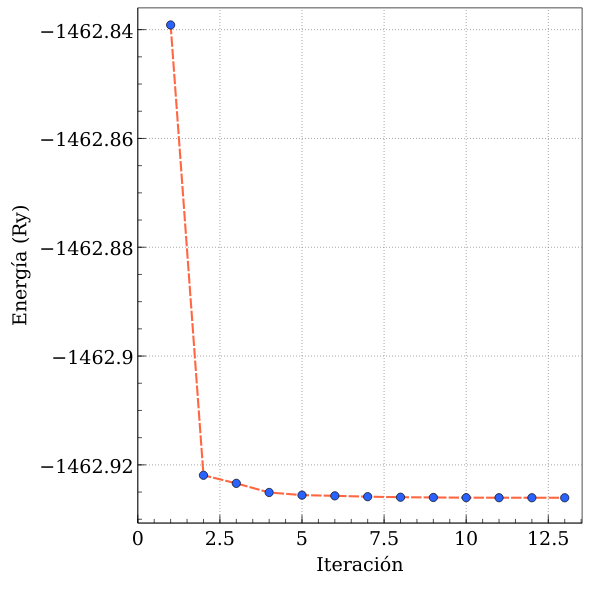
\includegraphics[width=0.9\textwidth]{contenido/resultados/img_resultados/energia_YCO_G.png}
            \caption{Minimizaci\'on de la energ\'ia del $YCrO_{3}$ con arreglo 
                antiferromagn\'etico tipo G.}
        \end{figure}
        \column{0.5\textwidth}
        \begin{figure}[H]
            \centering
            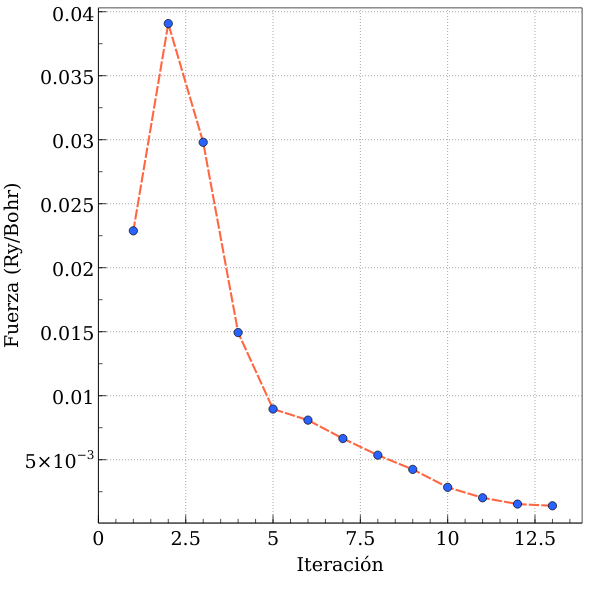
\includegraphics[width=0.9\textwidth]{contenido/resultados/img_resultados/fuerza_YCO_G.png}
            \caption{Minimizaci\'on de la fuerza del $YCrO_{3}$ con arreglo 
                antiferromagn\'etico tipo G.}
        \end{figure}
    \end{columns}
\centering
\textbf{El sistema converge luego de 13 iteraciones.}
\end{frame}